\documentclass[a4paper, 11pt, french]{report}
\usepackage[utf8]{inputenc}	% package désignant l'encodage
\usepackage[T1]{fontenc}	% je sais pas à quoi il sert
\usepackage[francais]{babel} % indique qu'on écrit en français
\usepackage{layout}	% Permet de gérer les marges
\usepackage[top=2cm, bottom=2cm, left=2cm, right=2cm]{geometry}	% Permet de définir les marges
\usepackage{graphicx}	% Insertion des images
\usepackage{setspace}
\usepackage{titlesec}
\titleformat{\chapter}[hang]{\bf\huge}{\thechapter}{2pc}{}
\usepackage{fancyhdr}	% Pour gérer les en-tête / pied de page
\usepackage{placeins}	% Pour utiliser \FloatBarrier qui annule les flottants
\usepackage{listings}	
\usepackage{hyperref}


\graphicspath{{img/}{../}}	% Définir l'emplacement des images

\makeatletter

\def\clap#1{\hbox to 0pt{\hss #1\hss}}%
\def\ligne#1
{%
\hbox to \hsize{%
\vbox{\centering #1}}
}%

\def\haut#1#2#3
{%
\hbox to \hsize{%
\rlap{\vtop{\raggedright #1}}%
\hss
\clap{\vtop{\centering #2}}%
\hss
\llap{\vtop{\raggedleft #3}}}
}%
\def\bas#1#2#3
{%
\hbox to \hsize{%
\rlap{\vbox{\raggedright #1}}%
\hss
\clap{\vbox{\centering #2}}%
\hss
\llap{\vbox{\raggedleft #3}}}
}%
\def\logo#1#2#3
{%
\hbox to \hsize{%
\rlap{\vbox{\raggedright #1}}%
\hss
\clap{\vbox{\centering #2}}%
\hss
\llap{\vbox{\raggedleft #3}}}
}%
\def\maketitle
{%
\thispagestyle{empty}\vbox to \vsize
{%
\begin{tabular}{lcr}
\hbox
{
\mbox{%
\hspace{4pt}%
%\includegraphics[scale=0.8]{Images/IUT.png}%}
\hspace{20pt}
}
}%
&
\hspace{5cm}
&
\raggedright
\hbox
{
\mbox{%
\hspace{20pt}%
%\includegraphics[scale=0.6]{Images/synergie.jpg}%
\hspace{4pt}
}
}%
\end{tabular}

\vspace{1cm}
\haut{}{\@blurb}{}

\vfill
%\vspace{1cm}
\begin{flushleft}
\huge \@title
\end{flushleft}
\par
\hrule height 2pt
\par
\begin{flushright}
\Large \@author
\par
\end{flushright}
%\vspace{1cm}
\vfill
\hbox
{
\mbox{%
\hspace{4pt}%
\logo{}{

\includegraphics[scale=1]{univ_nantes.jpg}%
}{}
\hspace{4pt}
}
}%
\vfill
\bas{}{\@location, le \@date}{}
}%
\cleardoublepage
}
\def\date#1{\def\@date{#1}}
\def\author#1{\def\@author{#1}}
\def\title#1{\def\@title{#1}}
\def\location#1{\def\@location{#1}}
\def\blurb#1{\def\@blurb{#1}}
\date{\today}
\author{}
%\title{Rapport de stage de deuxième année de DUT Informatique}
\location{Nantes}\blurb{}
\makeatother
\title{{\sl\LARGE\textbf{TP IHM - LoafMaker}}\normalsize}
\author{Guillaume Charon\\Jerôme Pages}
\blurb{%
Université de Nantes\\
UFR des Sciences et Techniques\\
Master ALMA 1
}


\begin{document}

	\pagestyle{plain}

	\maketitle	% Création de la page de garde
	\pagenumbering{arabic}

	\thispagestyle{empty}


	\renewcommand{\contentsname}{Sommaire} % Renomme la table des matières
	\setcounter{tocdepth}{2} % Définir la profondeur de la table des matières
	\addtocontents{toc}{%
	\protect\setlength{\baselineskip}{1.5em}	% Définir le saut de ligne dans la TDM
	\protect\setlength{\parskip}{0pt}	% Définir le saut de paragraphe dans la TDM
	}
	\tableofcontents\thispagestyle{plain}	% Table des matières
	%\pagenumbering{arabic}

	\begin{onehalfspace}
		%inclure le contenu
		\chapter{Noyau de l'application (Guillaume)}

	\section{Analyse}

		Structures de données et fonctionnalités
	
		-> Listes, sous-listes, tâches
		
	\section{Fonctionnalités}
	
		ghsdkglhsd
		
		


\chapter{Prototyping (Jerome)}

	\section{Storyboard}
		\begin{figure}[h!]
		   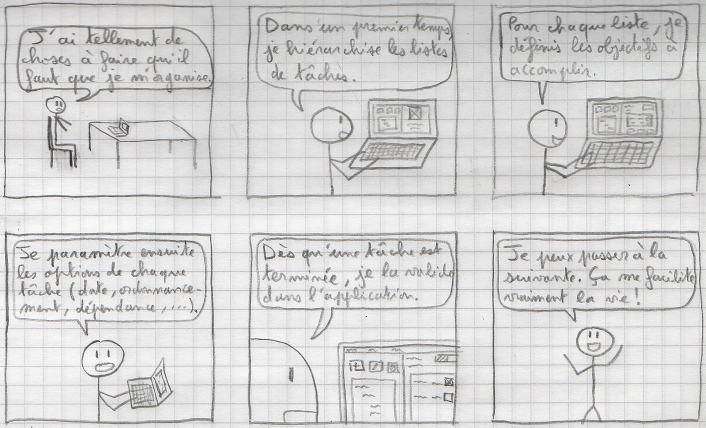
\includegraphics{img/stotyboard_ihm.png}
		   \caption{Storyboard de l'utilisation de l'application}
		\end{figure}
	
		La planche ci-dessus présente les différentes étapes d'utilisation basique du logiciel par un utilisateur lambda (son niveau de compétence n'entre pas ici en compte). Voici la liste des fonctionnalités évoquées et qui devront être présentes dans l'application finale :
		\begin{itemize}
			\item Création de listes imbriquées de tâches;
			\item Paramétrages possibles : dates relatives ou absolues, ordonnancement et dépendance des tâches;
			\item Validation des tâches et affichage de l'avancement;
			\item Sauvegarde en local des modifications effectuées.
		\end{itemize}
	
	\section{Paper-prototype}
	Une \href{https://www.youtube.com/watch?v=xbLaZvgkzjQ}{vidéo sur Youtube} est accessible pour montrer le fonctionnement de l'interface du prototype papier. Le rendu vidéo est en deça de ce à quoi nous nous attendions mais nous n'avons pas eu les conditions optimales (matérielles et logicielles) de production.
	
	
	

	\section{Scénarios d'utilisation}
	
	
	
	\section{Évaluation du prototype}
		Pour avoir un point de vue extérieur, nous avons demandé à un étudiant (qui a souhaité gardé l'anonymat) de nous donner son avis sur le prototype papier. Après plusieurs 
		On a demandé à Péneau ce qu'il pensait de notre paper-prototype, il a dit OK et on a modifié 2-3 trucs :)
		


\chapter{IHM}
	
	\section{Présentation (Guillaume)}
		screens
		dire que y a des popup pour confirmer la suppression (pas faire de caca) ou pour signaler à l'utilisateur que son action n'est pas possible (modifier une tache alors que y en a pas)
	
	\section{Ergonomie (Jerome)}
		Toute la difficulté pour la réalisation de l'interface graphique d'une telle application est de permettre de proposer à l'utilisateur néophyte un rendu clair et intuitif tout en proposant des fonctionnalités plus avancées pour un {\oe}il plus expert. Pour réussir cela, nous avons listé les différentes fonctionnalités souhaitées par ces deux groupes d'utilisateurs et les moyens possibles pour y arriver.
		
		Pour cela, nous avons décider de proposer plusieurs moyens d'arriver aux mêmes fonctionnalités. Par exemple, pour la création de tâches on peut passer par le menu de l'application, le bouton (+) sur la partie droite de l'écran, le clic droit sur cette même partie ou bien le raccourcis clavier. De cette manière, l'utilisateur aura toujours une solution qui lui conviendra plus que les autres et qu'il considèrera comme plus intuitive.
		
		De plus, nous avons choisi de toujours afficher le même menu pour ne pas perdre l'utilisateur avec des \og modes \fg d'utilisation. Ainsi, l'utilisateur aura toujours les mêmes repères visuels. Cela est important, en particulier pour les débutants, qui ne peuvent pas se raccrocher à leur expérience avec d'autres logiciels similaires.\newline
		
		Pour rendre l'utilisation plus intuitive, nous avons aussi décidé d'intégrer des icônes colorées, explicites et facilement reconnaissables pour limiter la quantité de texte à l'écran. Pour cela, nous avons utilisé des images tirées de la bibliothèque du projet \emph{Gnome}\footnote{\href{https://commons.wikimedia.org/wiki/GNOME_Desktop_icons}{Icônes disponibles ici.}} et disponibles sous licence GNU General Public License version 2. Les avantages de ces icônes sont nombreux : gratuits, libres, ergonomiques et disponibles en de nombreuses tailles, \dots \newline
		
		Nous avons souhaité permettre à l'utilisateur de contrôler dans une certaine mesure la taille des panneaux, c'est pourquoi nous avons permis d'agrandir l'un ou l'autre des côtés de la vue avec un /emph{splitter} vertical pour une meilleure lisibilité.
		
		En plus de cela, nous affichons une petite aide lors du lancement du programme pour permettre une prise en main rapide et aisée. En effet, le panneau dédié aux liste de tâche est temporairement remplacé par un message de bienvenue qui avertit l'utilisateur sur le fonctionnement du logiciel.
		
		
	\section{Structure des widgets (Guillaume)}
		
		
	
\chapter{Limites de l'application (TOUS)}
	


\chapter{Évaluations (TOUS)}
	
	Utilisateurs néophytes :
		Ma mère et ma soeur
		Ta mère
		
	Utilisateurs avancés :
		Pierre-Yves
		Leroux


	\end{onehalfspace}

\end{document}
